\begin{tcolorbox}
\chapter{2008 - Votla Gora}

2008 was the first ICCC Slovenia expedition with a name - `Votla
Gora', meaning `Hollow Mountain'. This was an idea, shamelessly copied from the recent OUCC Ario Caves expeditions, which instantly became a useful tradition.

The main focus of the Votla Gora expedition was the connection of \passage{Sistem Migovec} (at 11,493 m, the 5\(^{th}\) longest cave in Slovenia) with \passage{Vrtnarija} (5229 m - the 11\(^{th}\) longest). Connecting these caves would make the second longest cave in Slovenia, with a length of more than 16,722 m. The separation between the caves was 28 m on the centre line with many going leads.

The club attempted to connect \passage{Vrtnarija} to \passage{Sistem Migovec} at the bottom of \passage{M2}, the original deep cave pushed in the early 1970s by the Slovenian JSPDT. Below the epic \passage{Tolminski Silos} pitch (P120 m), the cave shut down into a series of small pitches with extremely tight rift, which had to be opened for passage with explosives. Exploration had finished in the 1970s at yet another such rift.

Although a connection between the two cave systems was not achieved, 1.2 km of cave passage was found and explored.

\end{tcolorbox}
\backgroundsetup{
    scale=1.1,
    color=black,
    opacity=1,
    angle=0,
    contents={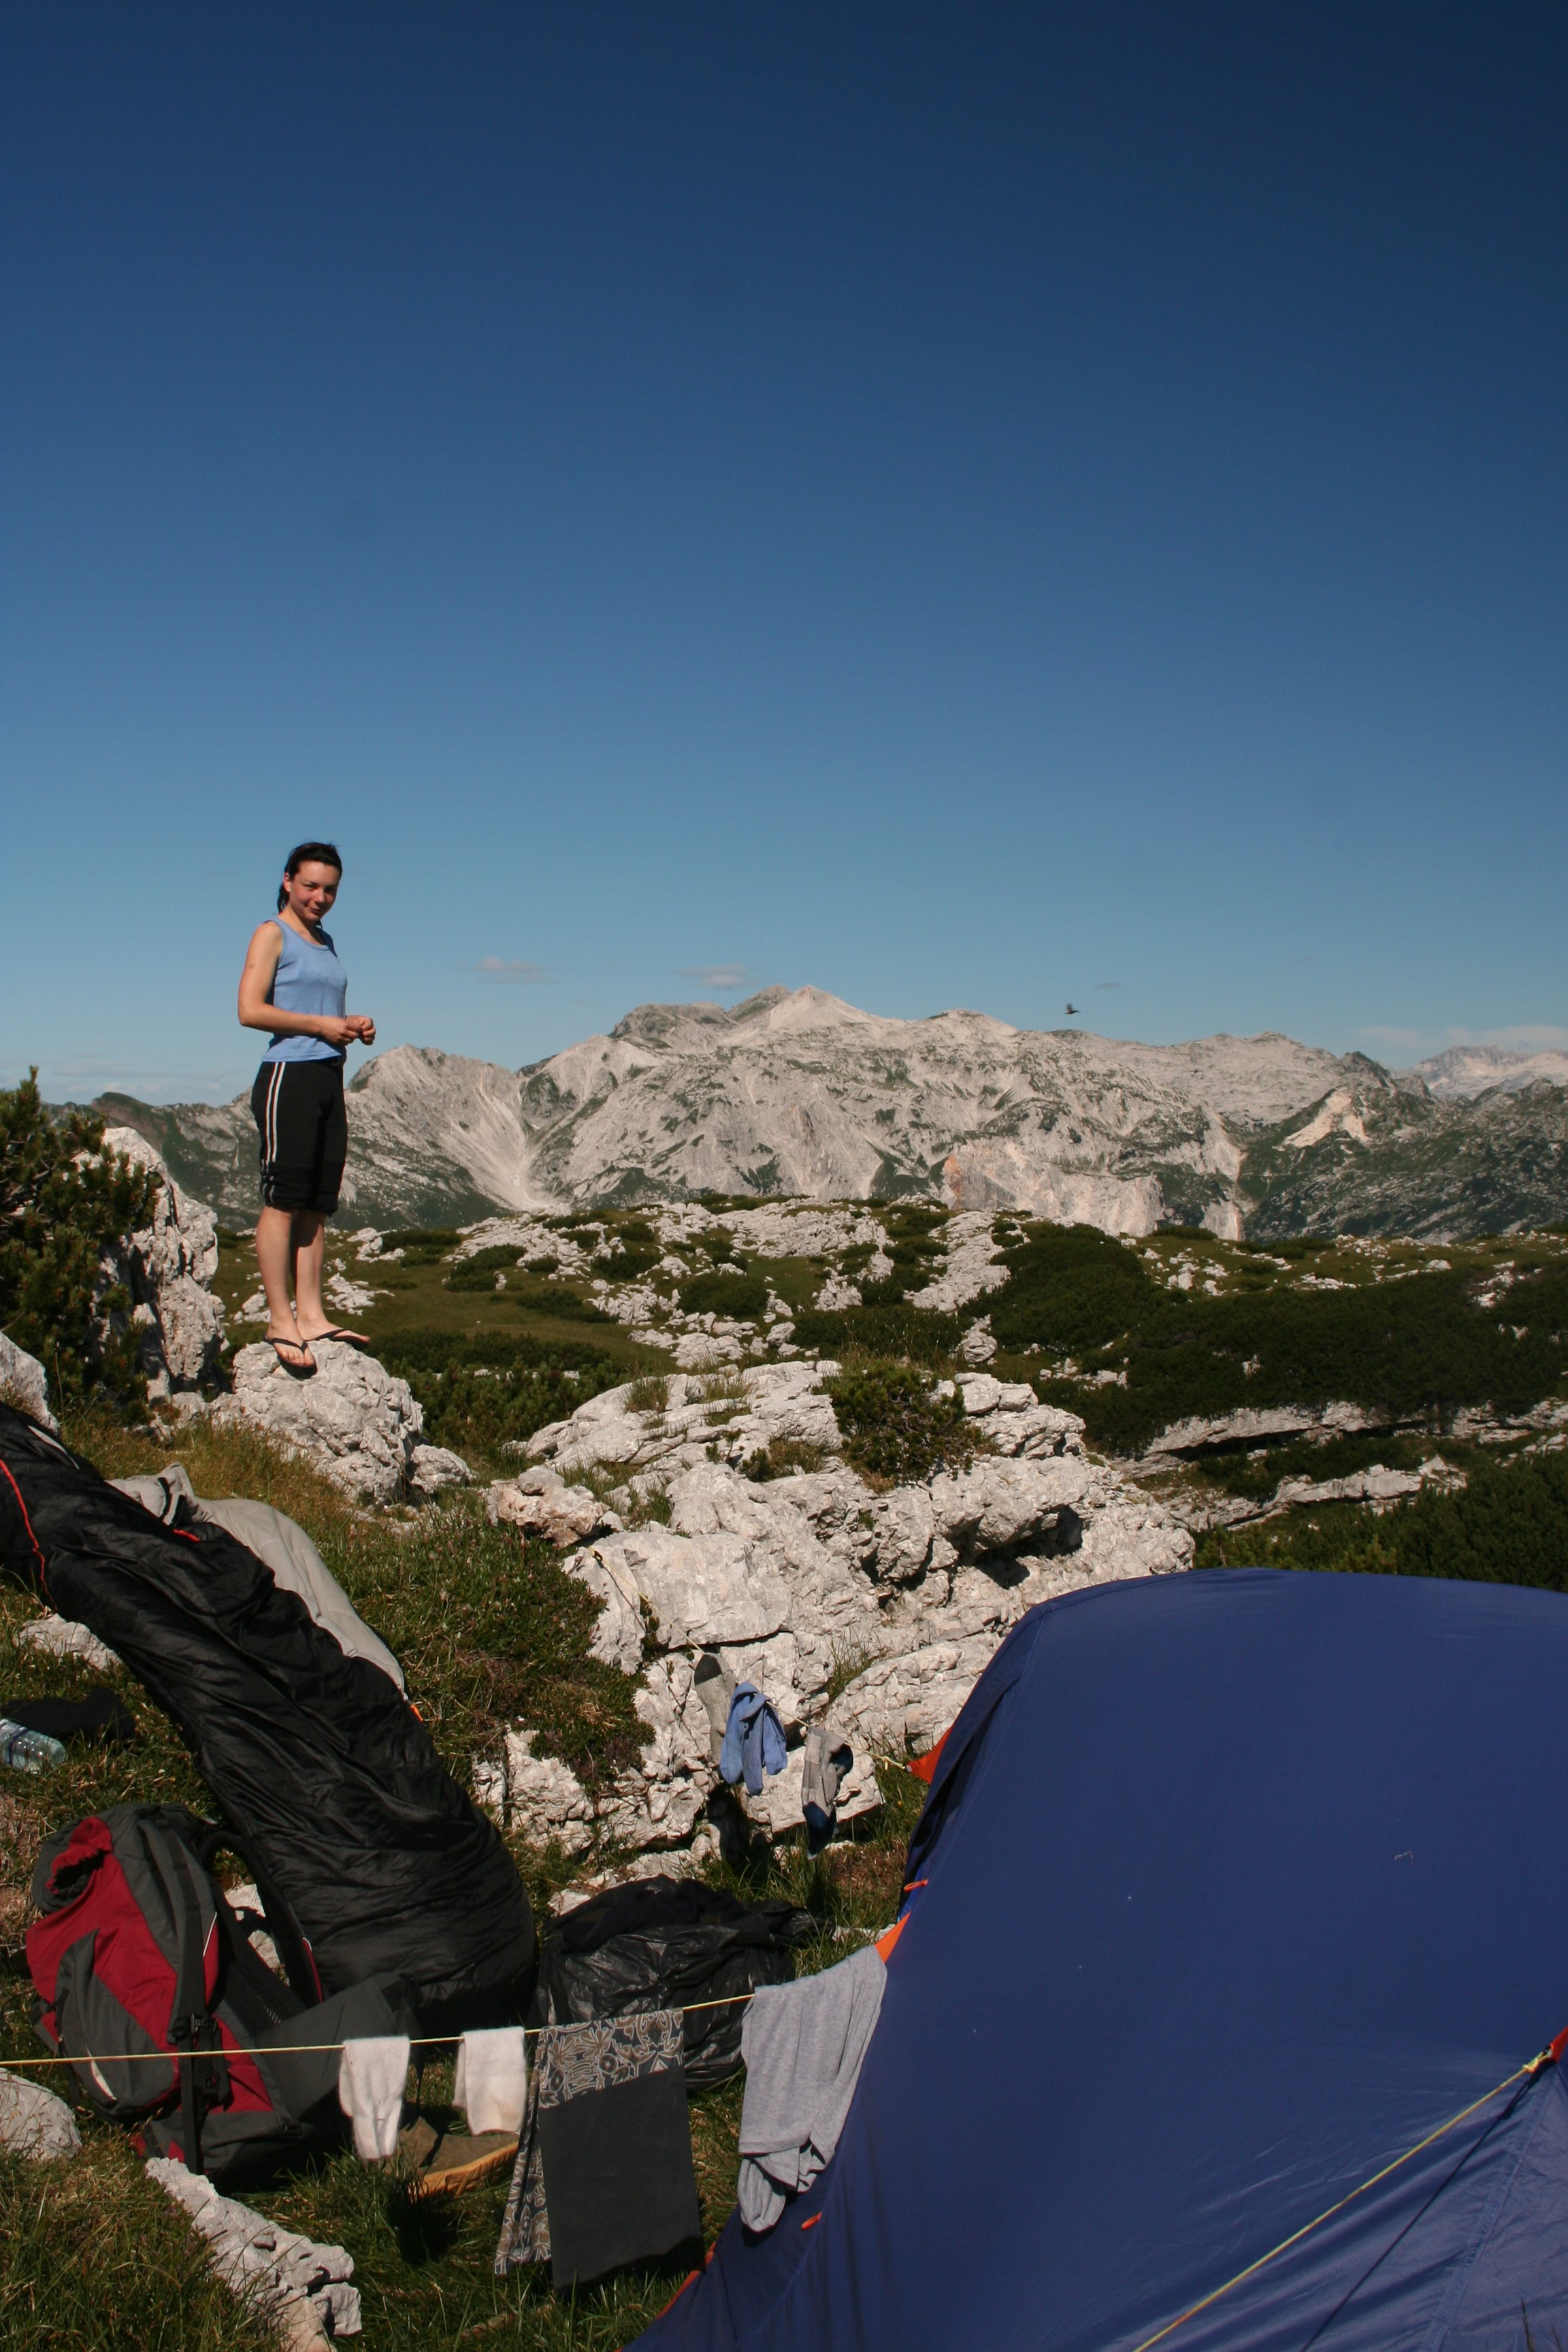
\includegraphics[height=\paperheight]{2008/intro/Jana Carga - Canon 350D - img_2998 jana posed by tent in morning on clear day.jpg}}
}
\BgThispage









